\documentclass{article}
\usepackage{graphicx}
\usepackage{booktabs}
\usepackage{hyperref}
\usepackage{listings}
\usepackage[margin=1in]{geometry}
\title{Autonomous Discovery of Bio-Plausible Learning Algorithms}
\author{AutoScientist}
\date{\today}
\begin{document}
\maketitle
\begin{abstract}
We present the results of an autonomous search for biologically plausible learning algorithms. Our system explored 1 configurations across multiple tasks. The top-performing model, Sparse Equilibrium, achieved 68.91\% accuracy.
\end{abstract}
\section{Introduction}
Deep learning relies on backpropagation, which is biologically implausible. Alternative algorithms such as Equilibrium Propagation \cite{scellier2017equilibrium} and Feedback Alignment \cite{lillicrap2016random} have been proposed.
\section{Methodology}
We utilized the AutoScientist framework to iteratively explore the hyperparameter space. Models were evaluated on tasks including Vision (MNIST/CIFAR) and Language Modeling.
\section{Chronicle of Discovery}
The following log details the autonomous decisions made by the scientist.
\begin{itemize}
\item \textbf{2026-02-04 20:06:57} [NEW_HYPOTHESIS]: Starting initial investigation (Smoke Test) for Backprop Baseline on tiny\_shakespeare.
\item \textbf{2026-02-04 20:06:57} [NEW_HYPOTHESIS]: Starting initial investigation (Smoke Test) for Backprop Baseline on mnist.
\item \textbf{2026-02-04 20:06:57} [NEW_HYPOTHESIS]: Starting initial investigation (Smoke Test) for EqProp MLP on mnist.
\item \textbf{2026-02-04 20:06:57} [NEW_HYPOTHESIS]: Starting initial investigation (Smoke Test) for Holomorphic EqProp on mnist.
\item \textbf{2026-02-04 20:06:57} [NEW_HYPOTHESIS]: Starting initial investigation (Smoke Test) for Directed EqProp (Deep EP) on mnist.
\item \textbf{2026-02-04 20:06:57} [NEW_HYPOTHESIS]: Starting initial investigation (Smoke Test) for Finite-Nudge EqProp on mnist.
\item \textbf{2026-02-04 20:06:57} [NEW_HYPOTHESIS]: Starting initial investigation (Smoke Test) for EqProp Diffusion on mnist.
\item \textbf{2026-02-04 20:06:57} [NEW_HYPOTHESIS]: Starting initial investigation (Smoke Test) for Neural Cube on mnist.
\item \textbf{2026-02-04 20:06:57} [NEW_HYPOTHESIS]: Starting initial investigation (Smoke Test) for Adaptive Feedback Alignment on mnist.
\item \textbf{2026-02-04 20:06:57} [NEW_HYPOTHESIS]: Starting initial investigation (Smoke Test) for Equilibrium Alignment on mnist.
\item \textbf{2026-02-04 20:06:57} [NEW_HYPOTHESIS]: Starting initial investigation (Smoke Test) for Layerwise Equilibrium FA on mnist.
\item \textbf{2026-02-04 20:06:57} [NEW_HYPOTHESIS]: Starting initial investigation (Smoke Test) for Energy Guided FA on mnist.
\item \textbf{2026-02-04 20:06:57} [NEW_HYPOTHESIS]: Starting initial investigation (Smoke Test) for Predictive Coding Hybrid on mnist.
\item \textbf{2026-02-04 20:06:57} [NEW_HYPOTHESIS]: Starting initial investigation (Smoke Test) for Sparse Equilibrium on mnist.
\item \textbf{2026-02-04 20:06:57} [NEW_HYPOTHESIS]: Starting initial investigation (Smoke Test) for Momentum Equilibrium on mnist.
\item \textbf{2026-02-04 20:06:57} [NEW_HYPOTHESIS]: Starting initial investigation (Smoke Test) for Stochastic FA on mnist.
\item \textbf{2026-02-04 20:06:57} [NEW_HYPOTHESIS]: Starting initial investigation (Smoke Test) for Energy Minimizing FA on mnist.
\item \textbf{2026-02-04 20:06:57} [NEW_HYPOTHESIS]: Starting initial investigation (Smoke Test) for DFA (Direct Feedback Alignment) on mnist.
\item \textbf{2026-02-04 20:06:57} [NEW_HYPOTHESIS]: Starting initial investigation (Smoke Test) for CHL (Contrastive Hebbian) on mnist.
\item \textbf{2026-02-04 20:06:57} [NEW_HYPOTHESIS]: Starting initial investigation (Smoke Test) for Deep Hebbian (Hundred-Layer) on mnist.
\item \textbf{2026-02-04 20:06:57} [NEW_HYPOTHESIS]: Starting initial investigation (Smoke Test) for EqProp Transformer (Attention Only) on tiny\_shakespeare.
\item \textbf{2026-02-04 20:06:57} [NEW_HYPOTHESIS]: Starting initial investigation (Smoke Test) for EqProp Transformer (Full) on tiny\_shakespeare.
\item \textbf{2026-02-04 20:06:57} [NEW_HYPOTHESIS]: Starting initial investigation (Smoke Test) for EqProp Transformer (Hybrid) on tiny\_shakespeare.
\item \textbf{2026-02-04 20:06:57} [NEW_HYPOTHESIS]: Starting initial investigation (Smoke Test) for EqProp Transformer (Recurrent) on tiny\_shakespeare.
\item \textbf{2026-02-04 20:07:33} [NEW_HYPOTHESIS]: Starting initial investigation (Smoke Test) for Sparse Equilibrium on cartpole.
\end{itemize}
\section{Results}
\subsection{Leaderboard}
\begin{table}[h]
\centering
\begin{tabular}{l c c}
\toprule
Model & Task & Accuracy \\
\midrule
Sparse Equilibrium & mnist & 68.91\% \\
\bottomrule
\end{tabular}
\caption{Top performing algorithms discovered by the system.}
\end{table}
\subsection{Analysis}
\begin{figure}[h]
\centering
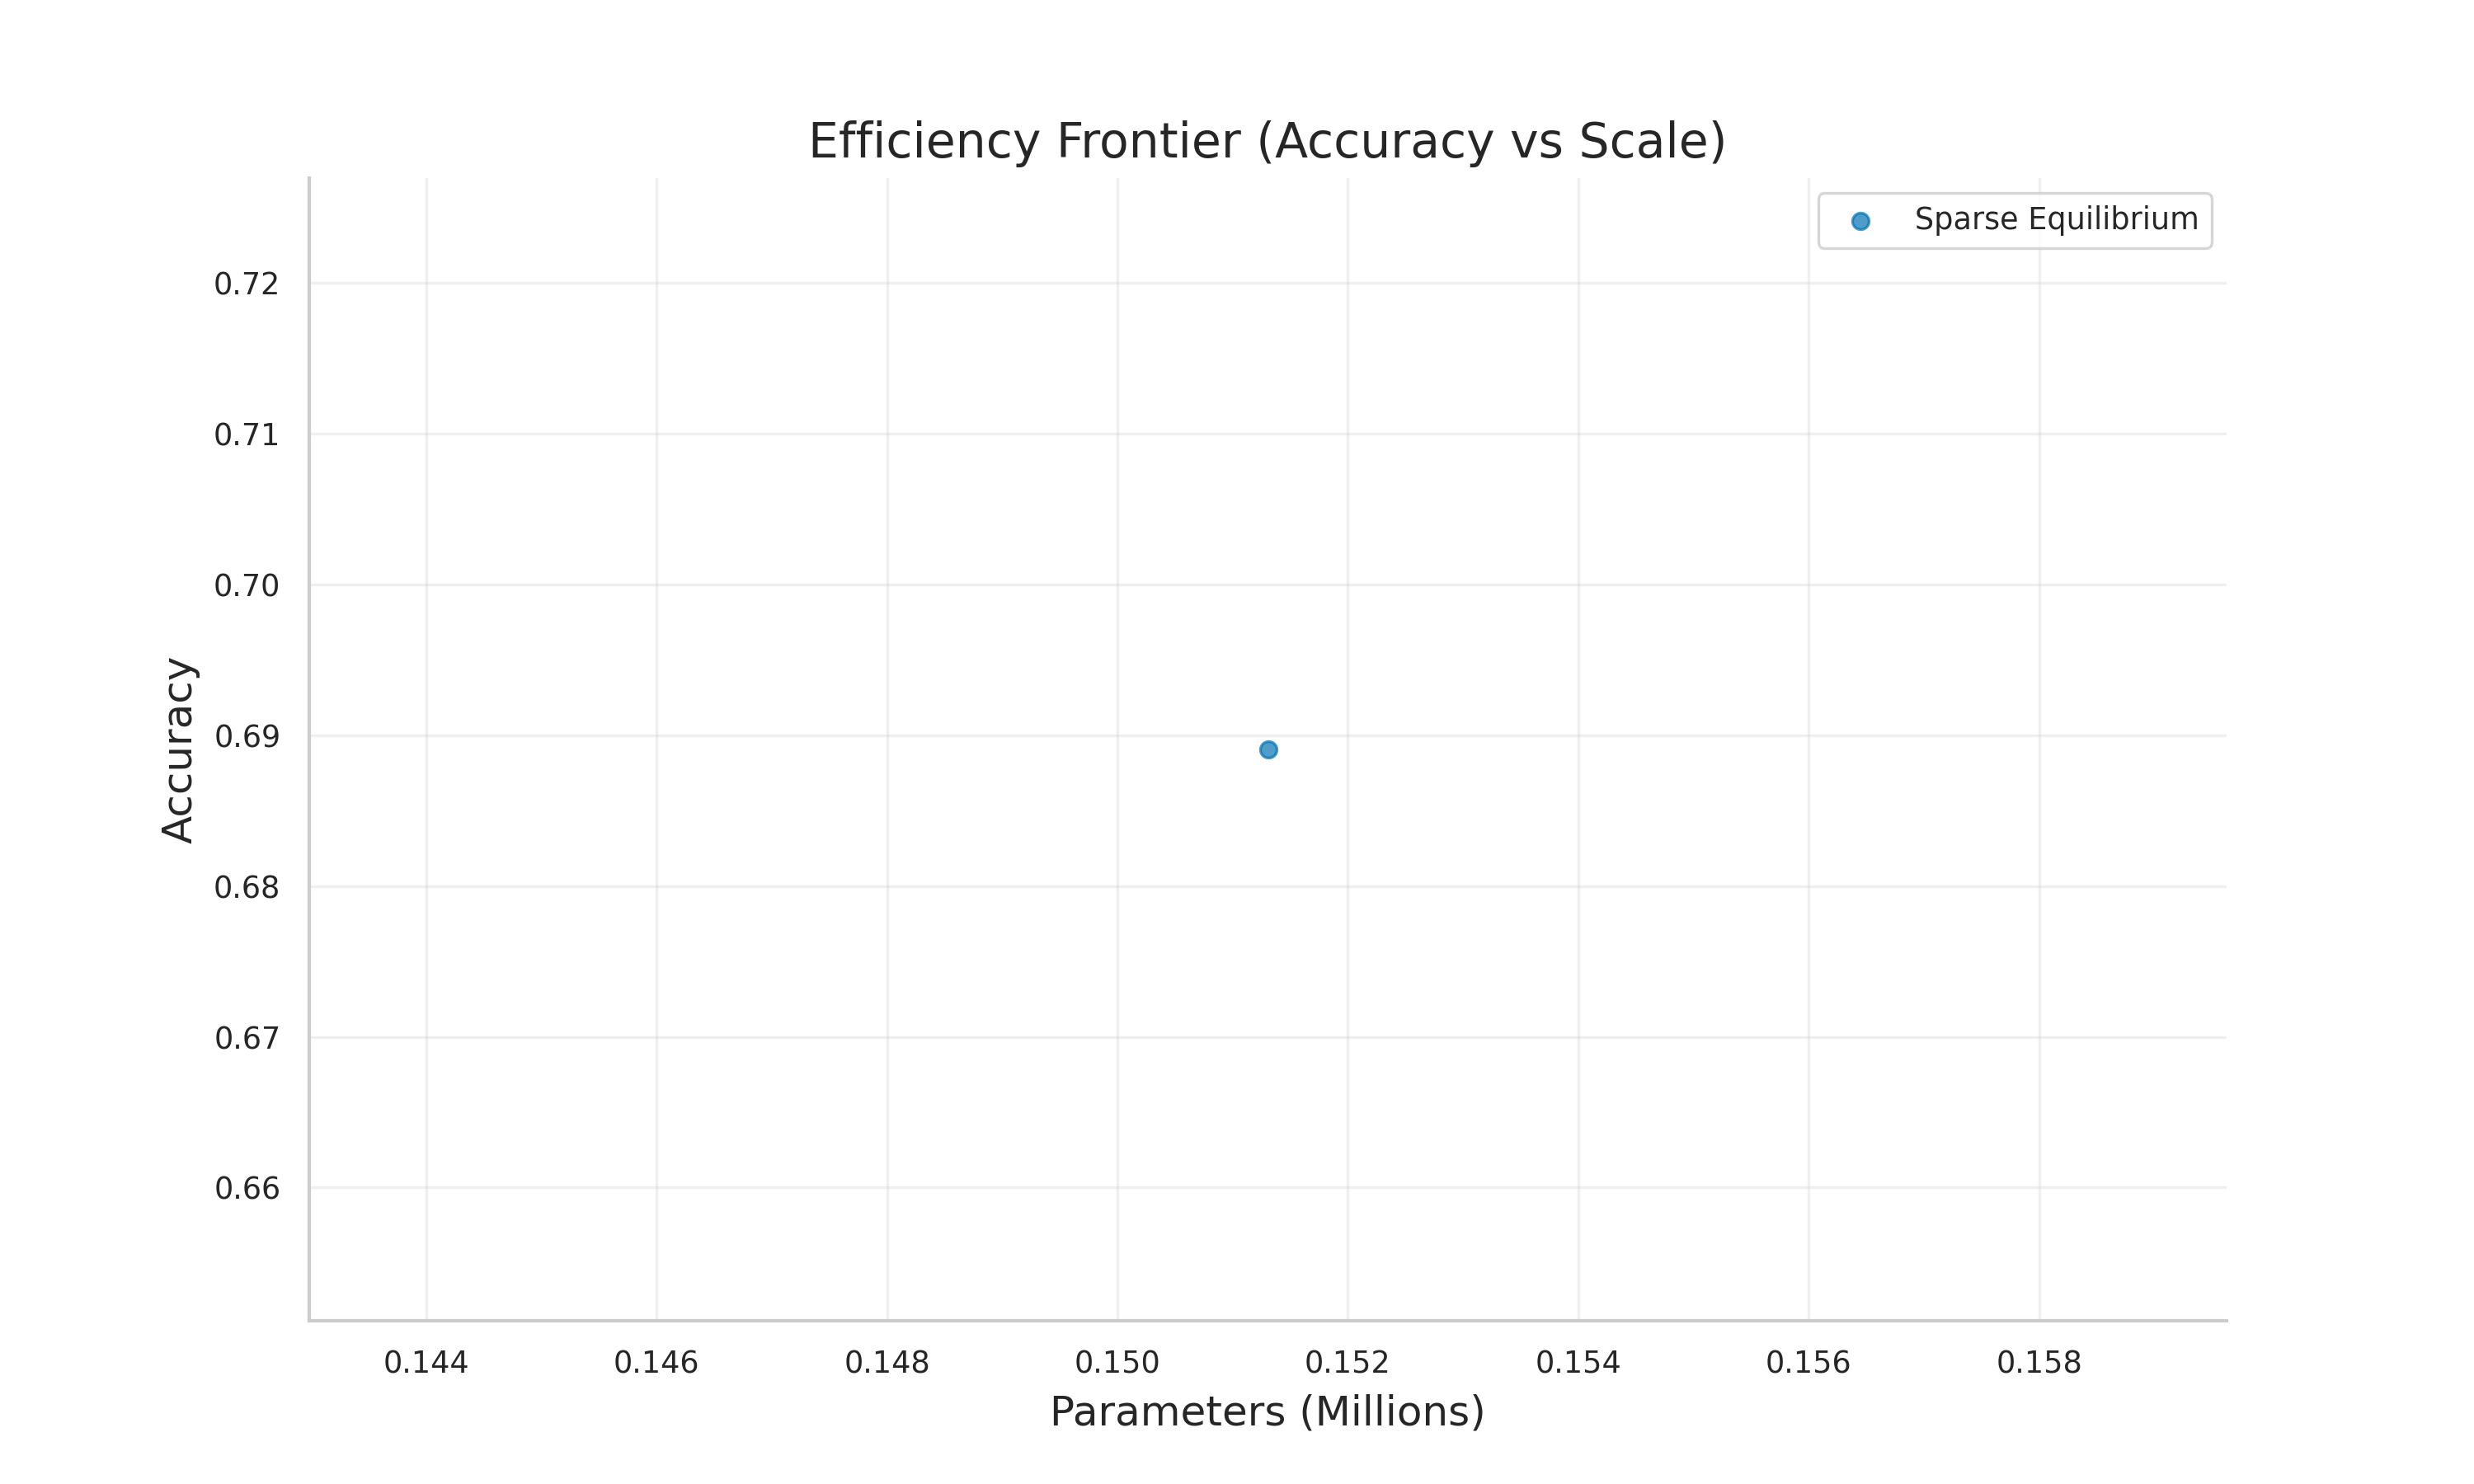
\includegraphics[width=0.8\textwidth]{images/pareto_frontier.png}
\caption{Pareto Frontier: Accuracy vs Parameter Efficiency.}
\end{figure}
\begin{figure}[h]
\centering
\includegraphics[width=0.8\textwidth]{images/significance_matrix.png}
\caption{Statistical Significance Matrix (P-Values).}
\end{figure}
\section{Machine Learning Analysis}
We utilized decision tree regression to interpret the experimental results.
No decision tree visualization available for the best model.
\bibliographystyle{plain}
\bibliography{references}
\appendix
\section{Best Configuration}
The hyperparameters for the top performing model are:
\begin{lstlisting}[basicstyle=\ttfamily\small, breaklines=true]
{
  "id": 1,
  "model": "Sparse Equilibrium",
  "accuracy": 0.6890625,
  "loss": 0.8734887367486954,
  "params": 0.151306,
  "lr": 0.007036310232029526,
  "beta": 0.230085244215255,
  "sparsity": 0.6934464408198258,
  "hidden_dim": 128,
  "epochs": 2,
  "batch_size": 256,
  "tier": "smoke",
  "task": "mnist",
  "job_id": 0
}
\end{lstlisting}
\end{document}